\specialsection{Обзор литературы}

В 1936 году Алан Тьюринг предложил модель формализации понятия алгоритма с помощью машины Тьюринга. На базе этой модели в работах [2, 3] были сформулированы первые подходы для оценки алгоритмов:
\begin{itemize}
\item оценка сложности программной реализации алгоритма;
\item оценка сложности вычислительного процесса, задаваемого алгоритмом.
\end{itemize}

В первом подходе оценку сложности связывают с качеством информации, которая содержится в записи алгоритма [4] или с объемом программной реализации алгоритма.
Во втором подходе для оценки сложности вычислительного процесса необходимо вводить меру сложности вычислений, задаваемых алгоритмом для решения конкретных задач. 

В зависимости от того, когда производится анализ (до или после реализации алгоритма), его можно разделить на два этапа:
\begin{enumerate}
\item Априорный (или теоретический) анализ — анализ алгоритма перед
его запуском на электронно-вычислительной машине.
\item Апостериорный (или экспериментальный) анализ — анализ алгоритма выполняется только после его запуска на электронно-вычислитель-
ной машине с определенными комплектующими.
\end{enumerate}

Априорный анализ использует только асимптотические оценки сложности алгоритма, зависящие от входных данных и их размеров. Методы априорного анализа хорошо представлены в работах [5, 6, 7].

Новый подход к анализу был предложен в работе [8] для повышения точности результатов эмпирического анализа алгоритма. Авторы фиксируют размер входных данных, проводят эксперименты и на основе собранных данных строят доверительный интервал функции трудоемкости алгоритма с заданным коэффициентом доверия. Для аппроксимации значений трудоемкости используется бета-распределение. Такой подход на практике показывает более реальные границы сложности алгоритма.

Описанный метод включает в себя два этапа:
\begin{enumerate}
\item предварительный этап — проверка гипотезы о законе распределения
трудоемкости алгоритма как ограниченной дискретной случайной величины [9];
\item основной этап — определение значения доверительной трудоемкости $f_{\gamma}(n)$ в зависимости от длины $n$ исследуемого алгоритма [8].
\end{enumerate}

\begin{figure}[h!]
\center{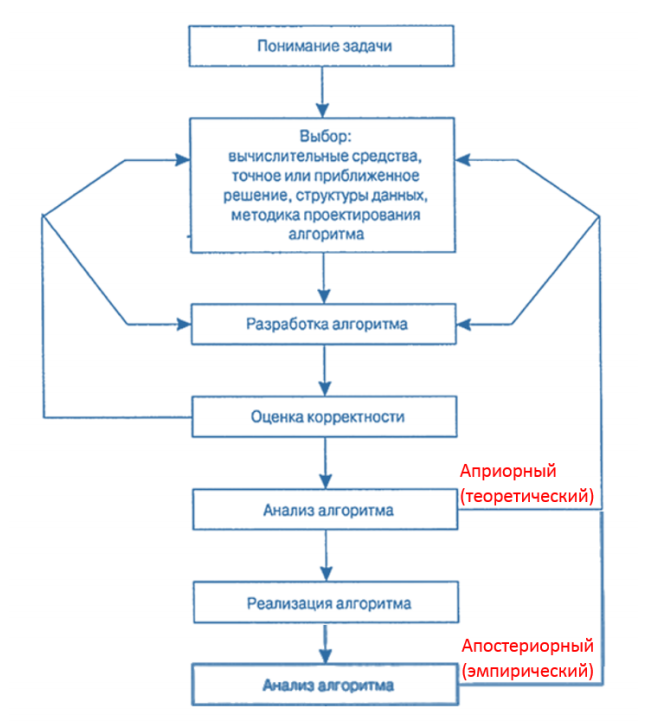
\includegraphics[width=0.7\linewidth]{images/scheme.png}}
\caption{Схема этапов при разработке алгоритма}
\label{ris:image1}
\end{figure}

За последние 10-15 лет машинное обучение вошло во множество научных и прикладных сфер. В частности методы машинного обучения были предложены для анализа сложности алгоритмов [10]. Можно ожидать, что в будущем эти методы будут дополняться и улучшаться.

Также стоит отметить, что в эпоху таких энергозатратных технологий как blockchain исследовать алгоритмы в апостериорном анализе можно не только на трудоемкость и ресурсоемкость, но также и на энергоэффективность [11]. В данный момент литературы по данной теме крайне мало.

\pagebreak